\documentclass[12pt,letterpaper]{article}
\usepackage{graphicx,textcomp}
\usepackage{natbib}
\usepackage{setspace}
\usepackage{fullpage}
\usepackage{color}
\usepackage[reqno]{amsmath}
\usepackage{amsthm}
\usepackage{fancyvrb}
\usepackage{amssymb,enumerate}
\usepackage[all]{xy}
\usepackage{endnotes}
\usepackage{lscape}
\newtheorem{com}{Comment}
\usepackage{float}
\usepackage{hyperref}
\newtheorem{lem} {Lemma}
\newtheorem{prop}{Proposition}
\newtheorem{thm}{Theorem}
\newtheorem{defn}{Definition}
\newtheorem{cor}{Corollary}
\newtheorem{obs}{Observation}
\usepackage[compact]{titlesec}
\usepackage{dcolumn}
\usepackage{tikz}
\usetikzlibrary{arrows}
\usepackage{multirow}
\usepackage{xcolor}
\newcolumntype{.}{D{.}{.}{-1}}
\newcolumntype{d}[1]{D{.}{.}{#1}}
\definecolor{light-gray}{gray}{0.65}
\usepackage{url}
\usepackage{listings}
\usepackage{color}

\definecolor{codegreen}{rgb}{0,0.6,0}
\definecolor{codegray}{rgb}{0.5,0.5,0.5}
\definecolor{codepurple}{rgb}{0.58,0,0.82}
\definecolor{backcolour}{rgb}{0.95,0.95,0.92}

\lstdefinestyle{mystyle}{
	backgroundcolor=\color{backcolour},   
	commentstyle=\color{codegreen},
	keywordstyle=\color{magenta},
	numberstyle=\tiny\color{codegray},
	stringstyle=\color{codepurple},
	basicstyle=\footnotesize,
	breakatwhitespace=false,         
	breaklines=true,                 
	captionpos=b,                    
	keepspaces=true,                 
	numbers=left,                    
	numbersep=5pt,                  
	showspaces=false,                
	showstringspaces=false,
	showtabs=false,                  
	tabsize=2
}
\lstset{style=mystyle}
\newcommand{\Sref}[1]{Section~\ref{#1}}
\newtheorem{hyp}{Hypothesis}

\title{Problem Set 3}
\date{Due: November 12, 2026}
\author{Elena Gyubin Lee}


\begin{document}
	\maketitle
	\section*{Instructions}
	\begin{itemize}
		\item Please show your work! You may lose points by simply writing in the answer. If the problem requires you to execute commands in \texttt{R}, please include the code you used to get your answers. Please also include the \texttt{.R} file that contains your code. If you are not sure if work needs to be shown for a particular problem, please ask.
	\item Your homework should be submitted electronically on GitHub.
	\item This problem set is due before 23:59 on Thursday November 12, 2026. No late assignments will be accepted.

	\end{itemize}

		\vspace{.25cm}
	
\noindent In this problem set, you will run several regressions and create an add variable plot (see the lecture slides) in \texttt{R} using the \texttt{incumbents\_subset.csv} dataset. Include all of your code.

\newpage

\section*{Question 1}
\vspace{.25cm}
\noindent We are interested in knowing how the difference in campaign spending between incumbent and challenger affects the incumbent's vote share. \vspace{.5cm}

	\begin{enumerate}
		
		% Q1.1
		\item \textbf{Run a regression where the outcome variable is \texttt{voteshare} and the explanatory variable is \texttt{difflog}.}	
		\vspace{.5cm}
			
			\lstinputlisting[language=R, firstline=44, lastline=45]{PS03_answers_EGL.R}
			\begin{verbatim}
				Call:
				lm(formula = voteshare ~ difflog, data = inc.sub)
				
				Residuals:
				Min       1Q   Median       3Q      Max 
				-0.26832 -0.05345 -0.00377  0.04780  0.32749 
				
				Coefficients:
				             Estimate Std. Error t value Pr(>|t|)    
				(Intercept) 0.579031   0.002251  257.19   <2e-16 ***
				difflog     0.041666   0.000968   43.04   <2e-16 ***
				---
				Signif. codes:  0 ‘***’ 0.001 ‘**’ 0.01 ‘*’ 0.05 ‘.’ 0.1 ‘ ’ 1
				
				Residual standard error: 0.07867 on 3191 degrees of freedom
				Multiple R-squared:  0.3673,	Adjusted R-squared:  0.3671 
				F-statistic:  1853 on 1 and 3191 DF,  p-value: < 2.2e-16
			\end{verbatim}
				
			\noindent When there is no log difference in campaign spending (the Y-intercept; \texttt{difflog} = 0) between the incumbent and challenger, the predicted vote share of the incumbent (henceforth '\textit{incumbent vote share}') is 0.579 ($\approx 57.9$ percentage points). 
			
			\noindent Each one-unit increase in log difference in campaign spending is associated with a 0.0417 increase ($\approx 4.2$ percentage points) in the predicted incumbent vote share, on average. 
			
			\noindent We also see that \texttt{difflog} is a statistically significant predictor of vote share at $\alpha = 0.001$ level ($t = 43$).
			
		\newpage
		% Q1.2
		\item \textbf{Make a scatterplot of the two variables and add the regression line.}	
			\vspace{.5cm}
			\lstinputlisting[language=R, firstline=51, lastline=54]{PS03_answers_EGL.R}
			\begin{figure} [H]
				\centering
				\caption{\footnotesize Incumbent vote share regressed on the log difference in campaign spending.}
				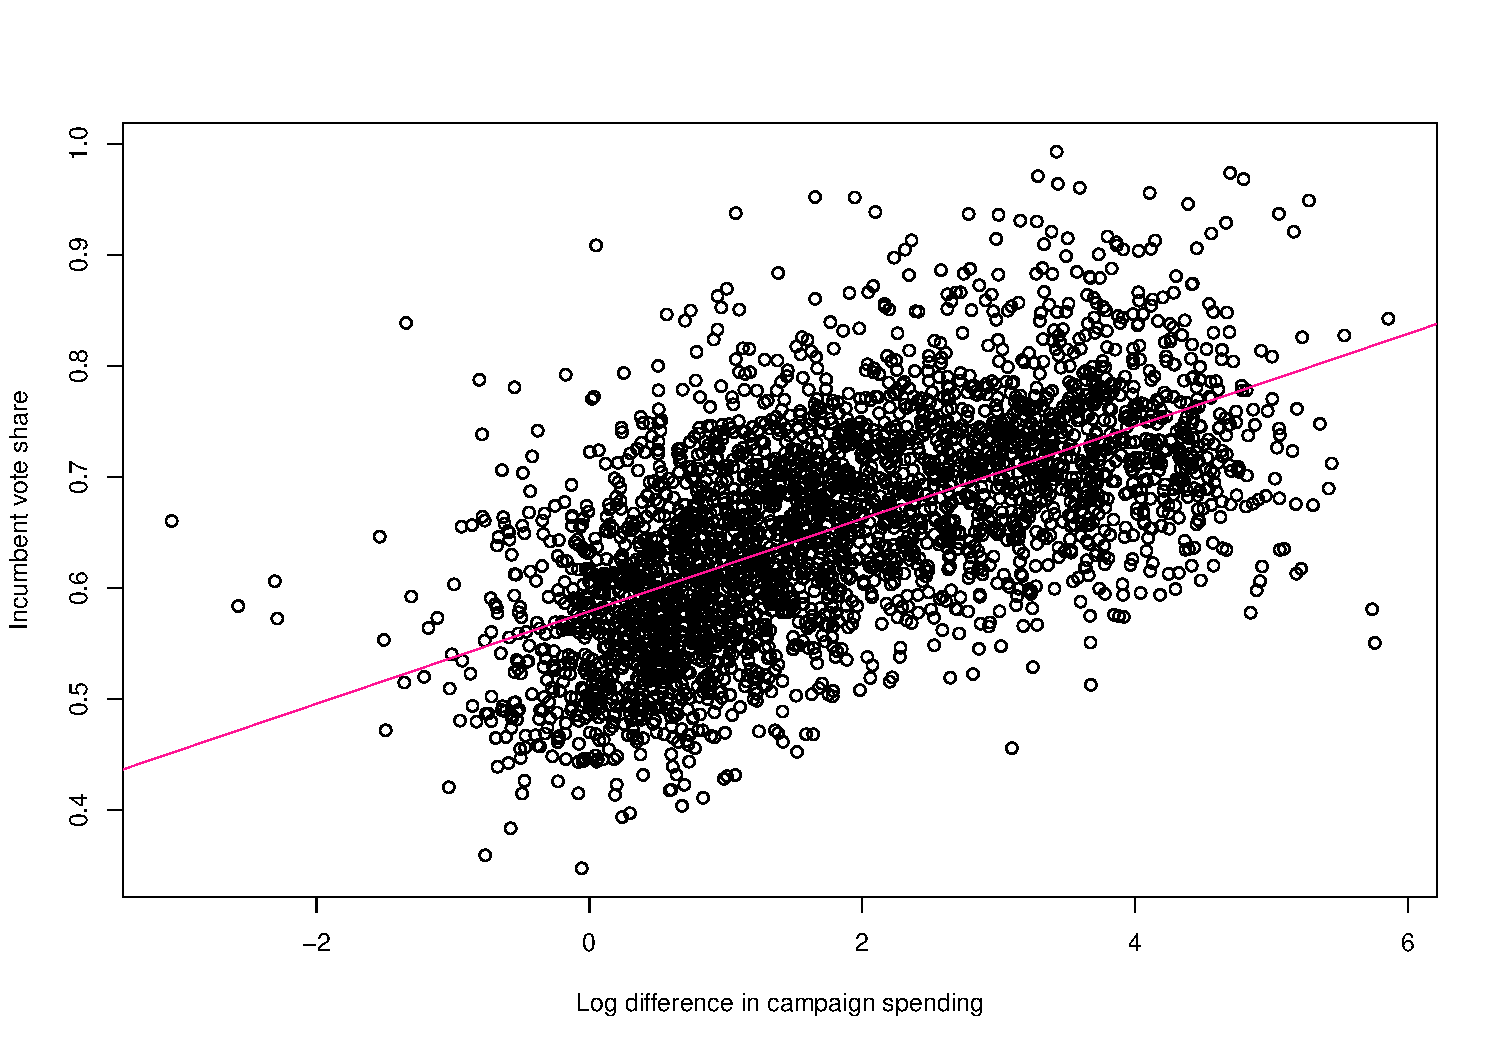
\includegraphics[width=1\textwidth]{SP_lm1.pdf}
			\end{figure}
			
		% Q1.3
		\item \textbf{Save the residuals of the model in a separate object.}
			\lstinputlisting[language=R, firstline=60, lastline=60]{PS03_answers_EGL.R}
		
		% Q1.4
		\item \textbf{Write the prediction equation.} 
		{\LARGE $$ \widehat{\text{voteshare}}_i = 0.579 + 0.042 \times \text{difflog}_i $$}
		\noindent $ \widehat{\text{incumbent vote share}}_i = 0.579 + 0.042 \times \text{log difference in campaign spending}_i $
		
	\end{enumerate}
	
\newpage

\section*{Question 2}
\noindent We are interested in knowing how the difference between incumbent and challenger's spending and the vote share of the presidential candidate of the incumbent's party are related.	\vspace{.25cm}
	
	\begin{enumerate}
		
		% Q2.1
		\item \textbf{Run a regression where the outcome variable is \texttt{presvote} and the explanatory variable is \texttt{difflog}.}	\vspace{.5cm}
			
		\lstinputlisting[language=R, firstline=74, lastline=75]{PS03_answers_EGL.R}
		\begin{verbatim}
			Call:
			lm(formula = presvote ~ difflog, data = inc.sub)
			
			Residuals:
			Min       1Q   Median       3Q      Max 
			-0.32196 -0.07407 -0.00102  0.07151  0.42743 
			
			Coefficients:
			             Estimate Std. Error t value Pr(>|t|)    
			(Intercept) 0.507583   0.003161  160.60   <2e-16 ***
			difflog     0.023837   0.001359   17.54   <2e-16 ***
			---
			Signif. codes:  0 ‘***’ 0.001 ‘**’ 0.01 ‘*’ 0.05 ‘.’ 0.1 ‘ ’ 1
			
			Residual standard error: 0.1104 on 3191 degrees of freedom
			Multiple R-squared:  0.08795,	Adjusted R-squared:  0.08767 
			F-statistic: 307.7 on 1 and 3191 DF,  p-value: < 2.2e-16
		\end{verbatim}
		
		\noindent When there is no log difference in campaign spending (Y-intercept; \texttt{difflog} = 0) between the incumbent and challenger, the predicted vote share for the presidential candidate of the incumbent's party (henceforth '\textit{presidential vote share}') is 0.508 ($\approx 50.8$ percentage points). 
		
		\noindent Each one-unit increase in log difference in campaign spending is associated, on average, with a 0.024 increase ($\approx 2.4$ percentage points) in the predicted presidential vote share. 
		
		\noindent We also see that \texttt{difflog} is a statistically significant predictor of vote share at $\alpha = 0.001$ level ($ t = 17.54$).
		
		\newpage
		% Q2.2 
		\item \textbf{Make a scatterplot of the two variables and add the regression line.}
		\vspace{.5cm}
			\lstinputlisting[language=R, firstline=80, lastline=83]{PS03_answers_EGL.R} 
			\begin{figure} [H]
				\centering 
				\caption{\footnotesize Presidential vote share regressed on the log difference in campaign spending.}
				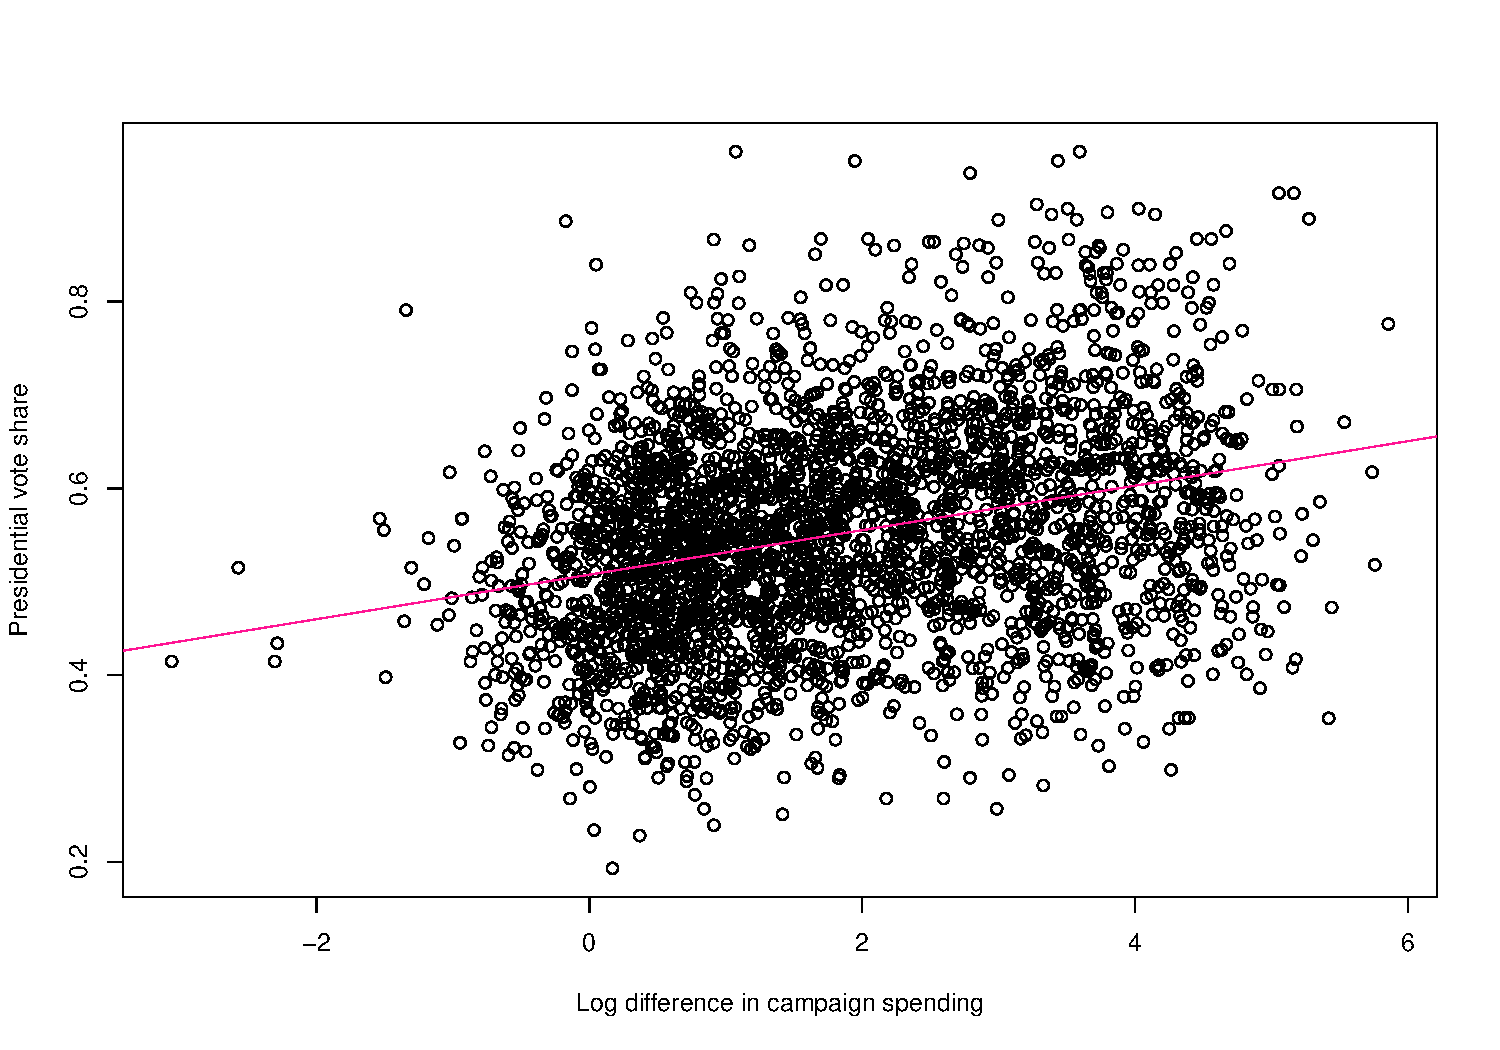
\includegraphics[width=1\textwidth]{SP_lm2.pdf}
			\end{figure}
		
		% Q2.3
		\item \textbf{Save the residuals of the model in a separate object.}
		\lstinputlisting[language=R, firstline=88, lastline=88]{PS03_answers_EGL.R} 		
		
		% Q2.4
		\item \textbf{Write the prediction equation.}
		{\LARGE $$ \widehat{\text{presvote}}_i = 0.508 + 0.024 \times \text{difflog}_i $$ }
		\noindent $ \widehat{\text{presidential vote share}}_i = 0.508 + 0.024 \times \text{log difference in campaign spending}_i $
		
	\end{enumerate}
		
	\newpage	
\section*{Question 3}

\noindent We are interested in knowing how the vote share of the presidential candidate of the incumbent's party is associated with the incumbent's electoral success.
\vspace{.25cm}
	
	\begin{enumerate}
		
		% Q3.1
		\item \textbf{Run a regression where the outcome variable is \texttt{voteshare} and the explanatory variable is \texttt{presvote}.} 
		
		\lstinputlisting[language=R, firstline=99, lastline=100]{PS03_answers_EGL.R}
		
		\begin{verbatim}
			Call:
			lm(formula = voteshare ~ presvote, data = inc.sub)
			
			Residuals:
			Min       1Q   Median       3Q      Max 
			-0.27330 -0.05888  0.00394  0.06148  0.41365 
			
			Coefficients:
			             Estimate Std. Error t value Pr(>|t|)    
			(Intercept) 0.441330   0.007599   58.08   <2e-16 ***
			presvote    0.388018   0.013493   28.76   <2e-16 ***
			---
			Signif. codes:  0 ‘***’ 0.001 ‘**’ 0.01 ‘*’ 0.05 ‘.’ 0.1 ‘ ’ 1
			
			Residual standard error: 0.08815 on 3191 degrees of freedom
			Multiple R-squared:  0.2058,	Adjusted R-squared:  0.2056 
			F-statistic:   827 on 1 and 3191 DF,  p-value: < 2.2e-16
		\end{verbatim}
		
		\noindent The intercept (0.441) is the predicted incumbent vote share when
		\texttt{presvote} = 0. Because a presidential candidate winning 0\% of the vote
		in a district is implausible and lies outside the observed range of the data, the
		intercept has no meaningful substantive interpretation.
		
		\noindent The slope indicates that a one-unit increase in presidential vote share is associated, on average, with a 0.388 increase in incumbent vote share. 
		
		\noindent But since both variables are measured as proportions (shares), a one-unit change would span the entire 0–1 range, which is not realistic. A more natural interpretation would be that a 1 percentage point (0.01 unit) increase in the presidential vote share is associated, on average, with a 0.39 percentage point (0.0039 units) increase in the incumbent vote share.
		
		\noindent We also see that \texttt{presvote} is statistically significant at the
		$\alpha = 0.001$ level ($t = 28.76$) and explains about 21\% of the variation in
		\texttt{voteshare} ($R^2 \approx 0.206$).
		
		\newpage
		% Q3.2
		\item \textbf{Make a scatterplot of the two variables and add the regression line.} 
		\vspace{.5cm}
		\lstinputlisting[language=R, firstline=105, lastline=108]{PS03_answers_EGL.R} 
			
		\begin{figure} [H]
			\centering 
			\caption{\footnotesize Incumbent vote share regressed on the presidential vote share.}
			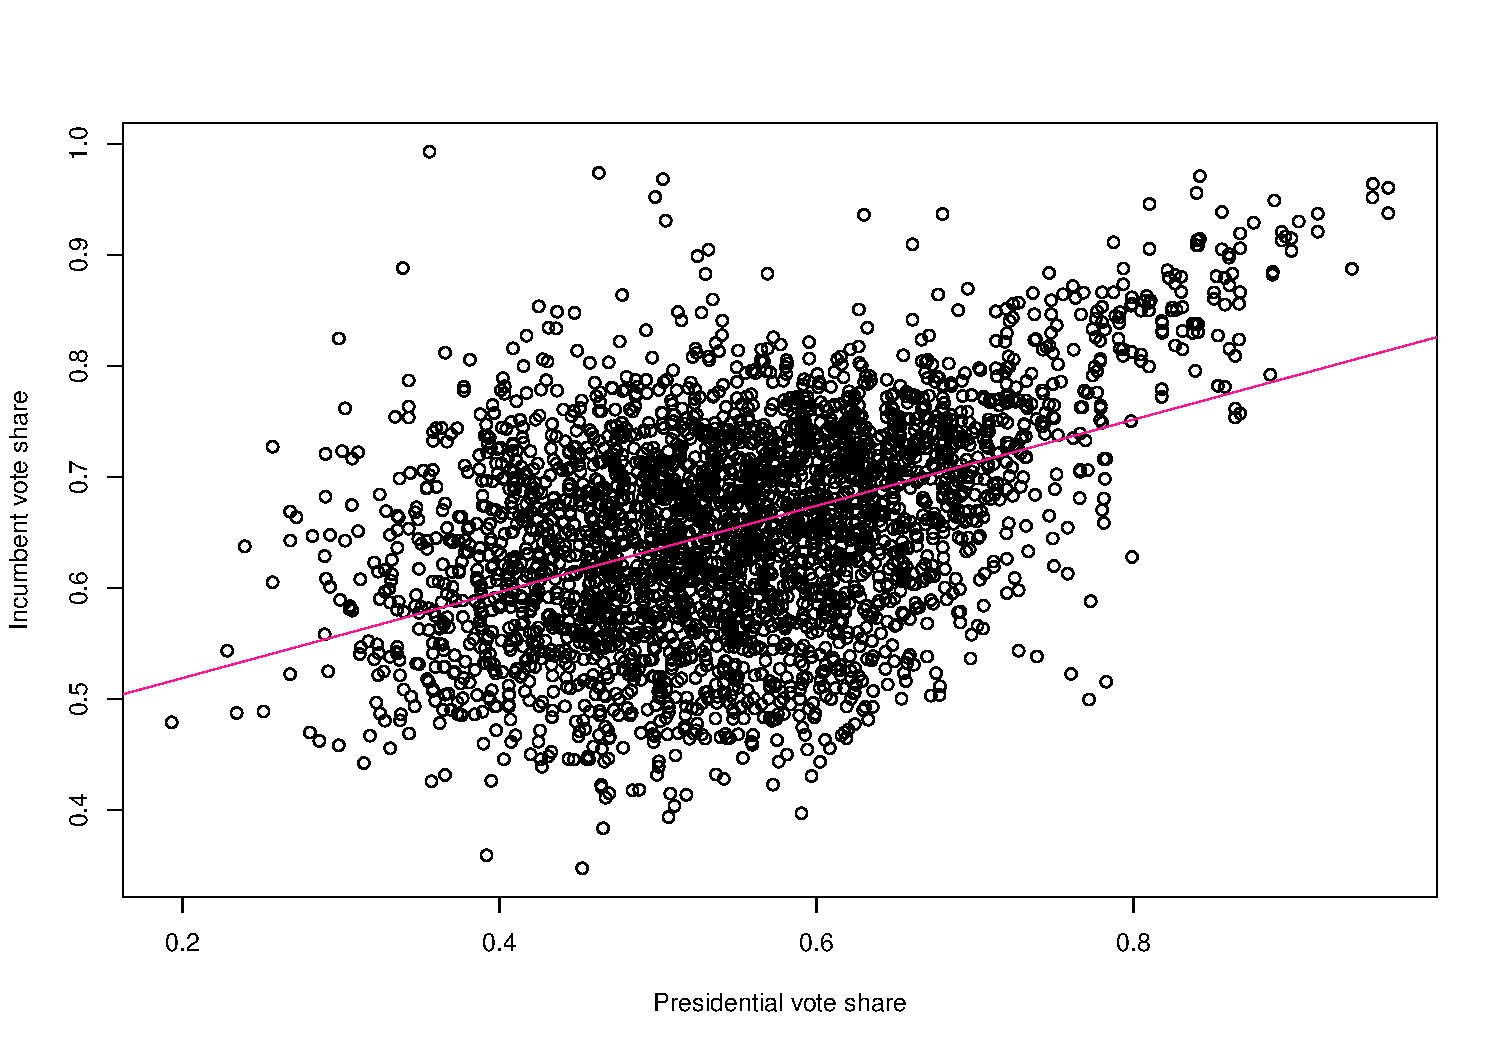
\includegraphics[width=1\textwidth]{SP_lm3.pdf}
		\end{figure}
			
		% Q3.3
		\item \textbf{Write the prediction equation.}
		{\LARGE $$ \widehat{\text{voteshare}}_i = 0.441 + 0.388 \times \text{presvote}_i $$ }
		\noindent $ \widehat{\text{incumbent vote share}}_i = 0.441 + 0.388 \times \text{presidential vote share}_i $
		
	\end{enumerate}
	

\newpage	
\section*{Question 4}
\noindent The residuals from part (a) tell us how much of the variation in \texttt{voteshare} is $not$ explained by the difference in spending between incumbent and challenger. The residuals in part (b) tell us how much of the variation in \texttt{presvote} is $not$ explained by the difference in spending between incumbent and challenger in the district.
	
	\begin{enumerate}
		% Q4.1
		\item \textbf{Run a regression where the outcome variable is the residuals from Question 1 and the explanatory variable is the residuals from Question 2.}
		\lstinputlisting[language=R, firstline=121, lastline=122]{PS03_answers_EGL.R}
		
		\begin{verbatim}
			Call:
			lm(formula = lm1_res ~ lm2_res)
			
			Residuals:
			Min       1Q   Median       3Q      Max 
			-0.25928 -0.04737 -0.00121  0.04618  0.33126 
			
			Coefficients:
			             Estimate Std. Error t value Pr(>|t|)    
			(Intercept) -1.942e-18  1.299e-03    0.00        1    
			lm2_res      2.569e-01  1.176e-02   21.84   <2e-16 ***
			---
			Signif. codes:  0 ‘***’ 0.001 ‘**’ 0.01 ‘*’ 0.05 ‘.’ 0.1 ‘ ’ 1
			
			Residual standard error: 0.07338 on 3191 degrees of freedom
			Multiple R-squared:   0.13,	Adjusted R-squared:  0.1298 
			F-statistic:   477 on 1 and 3191 DF,  p-value: < 2.2e-16
		\end{verbatim}
		
		\noindent The intercept is zero ($\approx -1.942 \times 10^{-18}$, rounding error). Because the residuals of \texttt{lm1} and \texttt{lm2} both sum to zero by construction, each set of residuals have a mean of 0. The intercept of Q4 regression is therefore $\hat\alpha = \bar{Y} - \hat\beta\bar{X} = 0 - \hat\beta \times 0 = 0$, which is reflected in the fitted line of \textit{Figure 4} passing through $(0, 0)$.
		
		\noindent After removing the linear association with \texttt{difflog} from both
		variables, a one-unit increase in the residual presidential vote share (the part
		not explained by \texttt{difflog}) is associated, on average, with a 0.257
		increase in the residual incumbent vote share. Put on a more realistic scale, a
		0.01 increase (1 percentage point) in the residual presidential vote share is
		associated with a 0.0026 increase (about 0.26 percentage points) in the residual
		incumbent vote share. 
		
		\noindent This relationship is statistically significant at the
		$\alpha = 0.001$ level. The residual presidential vote share
		explains about 13\% of the variation in the residual incumbent vote share
		($R^2 \approx 0.13$), i.e., 13\% of the variation in \texttt{voteshare} unexplained by
		\texttt{difflog}. \\
		
		% Q4.2
		\item \textbf{Make a scatterplot of the two residuals and add the regression line. }
		\lstinputlisting[language=R, firstline=127, lastline=130]{PS03_answers_EGL.R}
		
		\begin{figure} [H]
			\centering 
			\caption{\footnotesize Added variable plot for variation in vote share and presidential vote left unexplained by campaign spending.}
			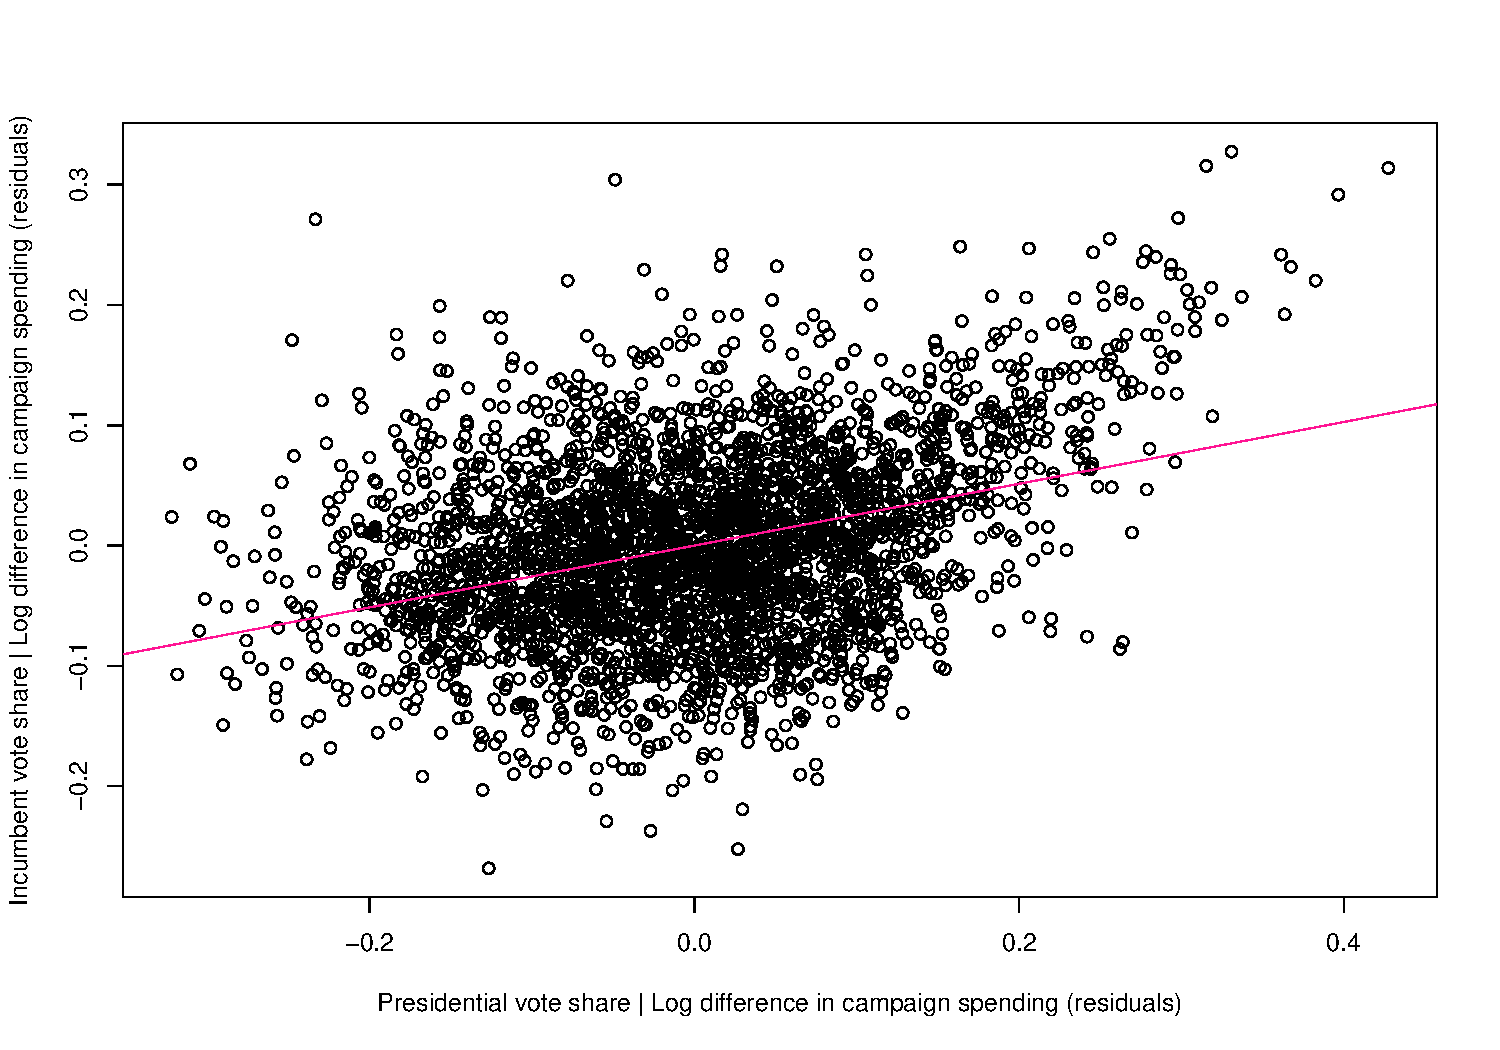
\includegraphics[width=0.95\textwidth]{SP_lm4.pdf}
		\end{figure}
		
		% 4.3
		\item \textbf{Write the prediction equation.}
			{\LARGE $$ \widehat{\text{lm1 res}}_i = 0 + 0.257 \times \text{lm2 res}_i $$ }
			\noindent $ \widehat{\text{residual incumbent vote share}}_i = 0 + 0.257  \times \text{residual presidential vote share}_i $
		
	\end{enumerate}
	
\newpage	
\section*{Question 5}
\noindent What if the incumbent's vote share is affected by both the president's popularity and the difference in spending between incumbent and challenger? 
	
	\begin{enumerate}
		% Q5.1
		\item \textbf{Run a regression where the outcome variable is the incumbent's \texttt{voteshare} and the explanatory variables are \texttt{difflog} and \texttt{presvote}.} 
		
			\lstinputlisting[language=R, firstline=143, lastline=144]{PS03_answers_EGL.R}
			
			\begin{verbatim}
				Call:
				lm(formula = voteshare ~ difflog + presvote, data = inc.sub)
				
				Residuals:
				Min       1Q   Median       3Q      Max 
				-0.25928 -0.04737 -0.00121  0.04618  0.33126 
				
				Coefficients:
				             Estimate Std. Error t value Pr(>|t|)        
				(Intercept) 0.4486442  0.0063297   70.88   <2e-16 ***
				difflog     0.0355431  0.0009455   37.59   <2e-16 ***
				presvote    0.2568770  0.0117637   21.84   <2e-16 ***
				---
				Signif. codes:  0 ‘***’ 0.001 ‘**’ 0.01 ‘*’ 0.05 ‘.’ 0.1 ‘ ’ 1
				
				Residual standard error: 0.07339 on 3190 degrees of freedom
				Multiple R-squared:  0.4496,	Adjusted R-squared:  0.4493 
				F-statistic:  1303 on 2 and 3190 DF,  p-value: < 2.2e-16
			\end{verbatim}
			
			\noindent The Y-intercept is not substantively meaningful because it is unlikely to find the presidential vote share at 0 and lies outside our observed data. 
			
			\noindent Keeping the presidential vote share constant, each one-unit increase in the log difference in campaign spending is associated with a 0.036 increase ($\approx 3.6$ percentage points) in the incumbent's vote share, on average. 
			
			\noindent Keeping the spending gap constant, each one-unit increase in the presidential vote share is associated with a 0.257 increase ($\approx 25.7 $ percentage points) in the incumbent vote share, on average. I.e., holding the spending gap constant, each 1 percentage point increase in the presidential vote share is associated with a 0.26 percentage point increase in the incumbent vote share. Both effects are statistically significant at the $\alpha = 0.001$ level (\texttt{difflog} at $t = 37.59$, \texttt{presvote} at $t = 21.84$). 
			
			\noindent Each coefficient is smaller than in its bivariate model: \texttt{difflog} falls from 0.042 (Q1, \texttt{lm1}) to 0.036, and \texttt{presvote} falls from 0.388 (Q3, \texttt{lm3}) to 0.257. This is consistent with Q2, where \texttt{difflog} had a significant positive association with \texttt{presvote}; the two predictors are positively associated with one another and with \texttt{voteshare}. Each bivariate model therefore attributed to its own predictor some variation that the other predictor also explains, and controlling for both removes this overlap.
			
			\noindent Together, the two variables explain about 45\% of the variation in the incumbent vote share ($R^2 \approx 0.450$; adjusted $R^2 \approx 0.449$), compared with an adjusted $R^2$ of 0.367 for \texttt{difflog} alone (Q1) and 0.206 for \texttt{presvote} alone (Q3). The two bivariate $R^2$ values sum to more than the joint value ($0.367 + 0.206 > 0.450$), which is consistent with that \texttt{difflog} and \texttt{presvote} explain overlapping variation in \texttt{voteshare}.
		\vspace{.5cm}
		
		% Q5.2
		\item \textbf{Write the prediction equation.}
			{\LARGE $$ \widehat{\text{voteshare}}_i = 0.449 + 0.036 \times \text{difflog}_i + 0.257 \times \text{presvote}_i $$}
			\noindent $\widehat{\text{incumbent vote share}}_i = 0.449 + (0.036 \times \text{log difference in campaign spending}_i) + (0.257 \times \text{presidential vote share}_i) $
			
		\vspace{1cm}
		% Q5.3
		\item \textbf{What is it in this output that is identical to the output in Question 4? Why do you think this is the case?} \vspace{.5cm}
		
		\noindent The \texttt{presvote} coefficient in the regression output above (0.257) and the \textit{t}-value (21.84) are identical to the slope of Q4's regression output, which aligns with our lecture expectations that the slope of the added-variable plot equals the multivariate $\beta$.
		
		\noindent This is because both models try to estimate how much the incumbent’s vote share changes with the presidential candidate's vote share, holding campaign spending constant. Question 4 does this in two steps: it calculates the residuals, removing the part of each variable explained by \texttt{difflog}, then regresses residual on residual. Q5 does it in
		one step, estimating both coefficients simultaneously through the multivariate regression.
		
	\end{enumerate}
	
\newpage
\section*{Appendix}
\noindent The above is visually encapsulated using the \texttt{stargazer} package, where we can see the models side by side.
\vspace{.5cm}
	
	\begin{table}[h] \centering 
		\caption{Incumbent vote share (bivariate and multiple regressions)} 
		\label{} 
		\small 
		\begin{tabular}{@{\extracolsep{3pt}}lccc} 
			\\[-1.8ex]\hline 
			\hline \\[-1.8ex] 
			& \multicolumn{3}{c}{\textit{Dependent variable:}} \\ 
			\cline{2-4} 
			\\[-1.8ex] & \multicolumn{3}{c}{Incumbent vote share} \\ 
			\\[-1.8ex] & (1) & (2) & (3)\\ 
			\hline \\[-1.8ex] 
			Log spending difference & 0.042$^{***}$ &  & 0.036$^{***}$ \\ 
			& (0.001) &  & (0.001) \\ 
			& & & \\ 
			Presidential vote share &  & 0.388$^{***}$ & 0.257$^{***}$ \\ 
			&  & (0.013) & (0.012) \\ 
			& & & \\ 
			Constant & 0.579$^{***}$ & 0.441$^{***}$ & 0.449$^{***}$ \\ 
			& (0.002) & (0.008) & (0.006) \\ 
			& & & \\ 
			\hline \\[-1.8ex] 
			Observations & 3,193 & 3,193 & 3,193 \\ 
			R$^{2}$ & 0.367 & 0.206 & 0.450 \\ 
			Adjusted R$^{2}$ & 0.367 & 0.206 & 0.449 \\ 
			Residual Std. Error & 0.079 (df = 3191) & 0.088 (df = 3191) & 0.073 (df = 3190) \\ 
			\hline 
			\hline \\[-1.8ex] 
			\textit{Note:}  & \multicolumn{3}{r}{$^{*}$p$<$0.1; $^{**}$p$<$0.05; $^{***}$p$<$0.01} \\ 
		\end{tabular} 
	\end{table} 
	
	\vspace{1.5cm}
	\noindent Styled with the help of stack overflow and \href{https://cran.r-project.org/web/packages/stargazer/vignettes/stargazer.pdf}{CRAN}.
	\lstinputlisting[language=R, firstline=157, lastline=168]{PS03_answers_EGL.R}
	
	
\end{document}
